%%%%%%%%%%%%%%%%%%%%%%%%%%%%%%%%%%%%%%%%%
% Short Sectioned Assignment
% LaTeX Template
% Version 1.0 (5/5/12)
%
% This template has been downloaded from:
% http://www.LaTeXTemplates.com
%
% Original author:
% Frits Wenneker (http://www.howtotex.com)
%
% License:
% CC BY-NC-SA 3.0 (http://creativecommons.org/licenses/by-nc-sa/3.0/)
%
%%%%%%%%%%%%%%%%%%%%%%%%%%%%%%%%%%%%%%%%%

%----------------------------------------------------------------------------------------
%	PACKAGES AND OTHER DOCUMENT CONFIGURATIONS
%----------------------------------------------------------------------------------------

\documentclass[paper=a4, fontsize=11pt]{scrartcl} % A4 paper and 11pt font size

\usepackage[T1]{fontenc} % Use 8-bit encoding that has 256 glyphs
\usepackage{fourier} % Use the Adobe Utopia font for the document - comment this line to return to the LaTeX default
\usepackage[english]{babel} % English language/hyphenation
\usepackage{amsmath,amsfonts,amsthm} % Math packages

\usepackage{lipsum} % Used for inserting dummy 'Lorem ipsum' text into the template

\usepackage{graphicx}
\usepackage{subcaption}
\usepackage{hyperref}
\usepackage[utf8]{inputenc} 

\usepackage[toc,page]{appendix} 

\usepackage{sectsty} % Allows customizing section commands
\allsectionsfont{\centering \normalfont\scshape} % Make all sections centered, the default font and small caps

\usepackage{fancyhdr} % Custom headers and footers
\pagestyle{fancyplain} % Makes all pages in the document conform to the custom headers and footers
\fancyhead{} % No page header - if you want one, create it in the same way as the footers below
\fancyfoot[L]{} % Empty left footer
\fancyfoot[C]{} % Empty center footer
\fancyfoot[R]{\thepage} % Page numbering for right footer
\renewcommand{\headrulewidth}{0pt} % Remove header underlines
\renewcommand{\footrulewidth}{0pt} % Remove footer underlines
\setlength{\headheight}{13.6pt} % Customize the height of the header

\numberwithin{equation}{section} % Number equations within sections (i.e. 1.1, 1.2, 2.1, 2.2 instead of 1, 2, 3, 4)
\numberwithin{figure}{section} % Number figures within sections (i.e. 1.1, 1.2, 2.1, 2.2 instead of 1, 2, 3, 4)
\numberwithin{table}{section} % Number tables within sections (i.e. 1.1, 1.2, 2.1, 2.2 instead of 1, 2, 3, 4)

\setlength\parindent{0pt} % Removes all indentation from paragraphs - comment this line for an assignment with lots of text

%----------------------------------------------------------------------------------------
%	TITLE SECTION
%----------------------------------------------------------------------------------------

\newcommand{\horrule}[1]{\rule{\linewidth}{#1}} % Create horizontal rule command with 1 argument of height

\title{	
\normalfont \normalsize 
\textsc{Aalborg University, School of Information and Communication Technology} \\ [25pt] % Your university, school and/or department name(s)
\horrule{0.5pt} \\[0.4cm] % Thin top horizontal rule
\huge Operation Observation \\ % The assignment title
\horrule{2pt} \\[0.5cm] % Thick bottom horizontal rule
}

\date{\normalsize\today} % Today's date or a custom date

\begin{document}

\maketitle % Print the title

%----------------------------------------------------------------------------------------
%	PROBLEM 1
%----------------------------------------------------------------------------------------

\section{Purpose}
The purpose of the observation is to observe the situation which must be simulated. This is done to make an assessment of what must be included in the design.  

\section{Method}
To analyse and retrieve information in the matter the main method used is doing a contextual inquiry. This includes the different analysing models and interviews. A group of three was at Aalborg University Hospital to observe a robot assisted surgery performed on a person.

The observation team acquired both pictures, notes and some video from the operation. Which describes the tasks and teamwork necessary to perform such an operation. From this different models used in contextual inquiries are made. The models used are a physical model showing the layout of the room, a sequence model to clarify the work needed to be done and an artefact model showing what is used together with the robot.

\section{Results}
The physical model shows the layout of the entire operation room and where the nurses move. This gives an overview of the operation room and how each nurse acts in the room. The figure includes doors and their movement as well as cabinets. The layout is shown in \autoref{fig:layout}.

\begin{figure}[hpbt]
	\centering
	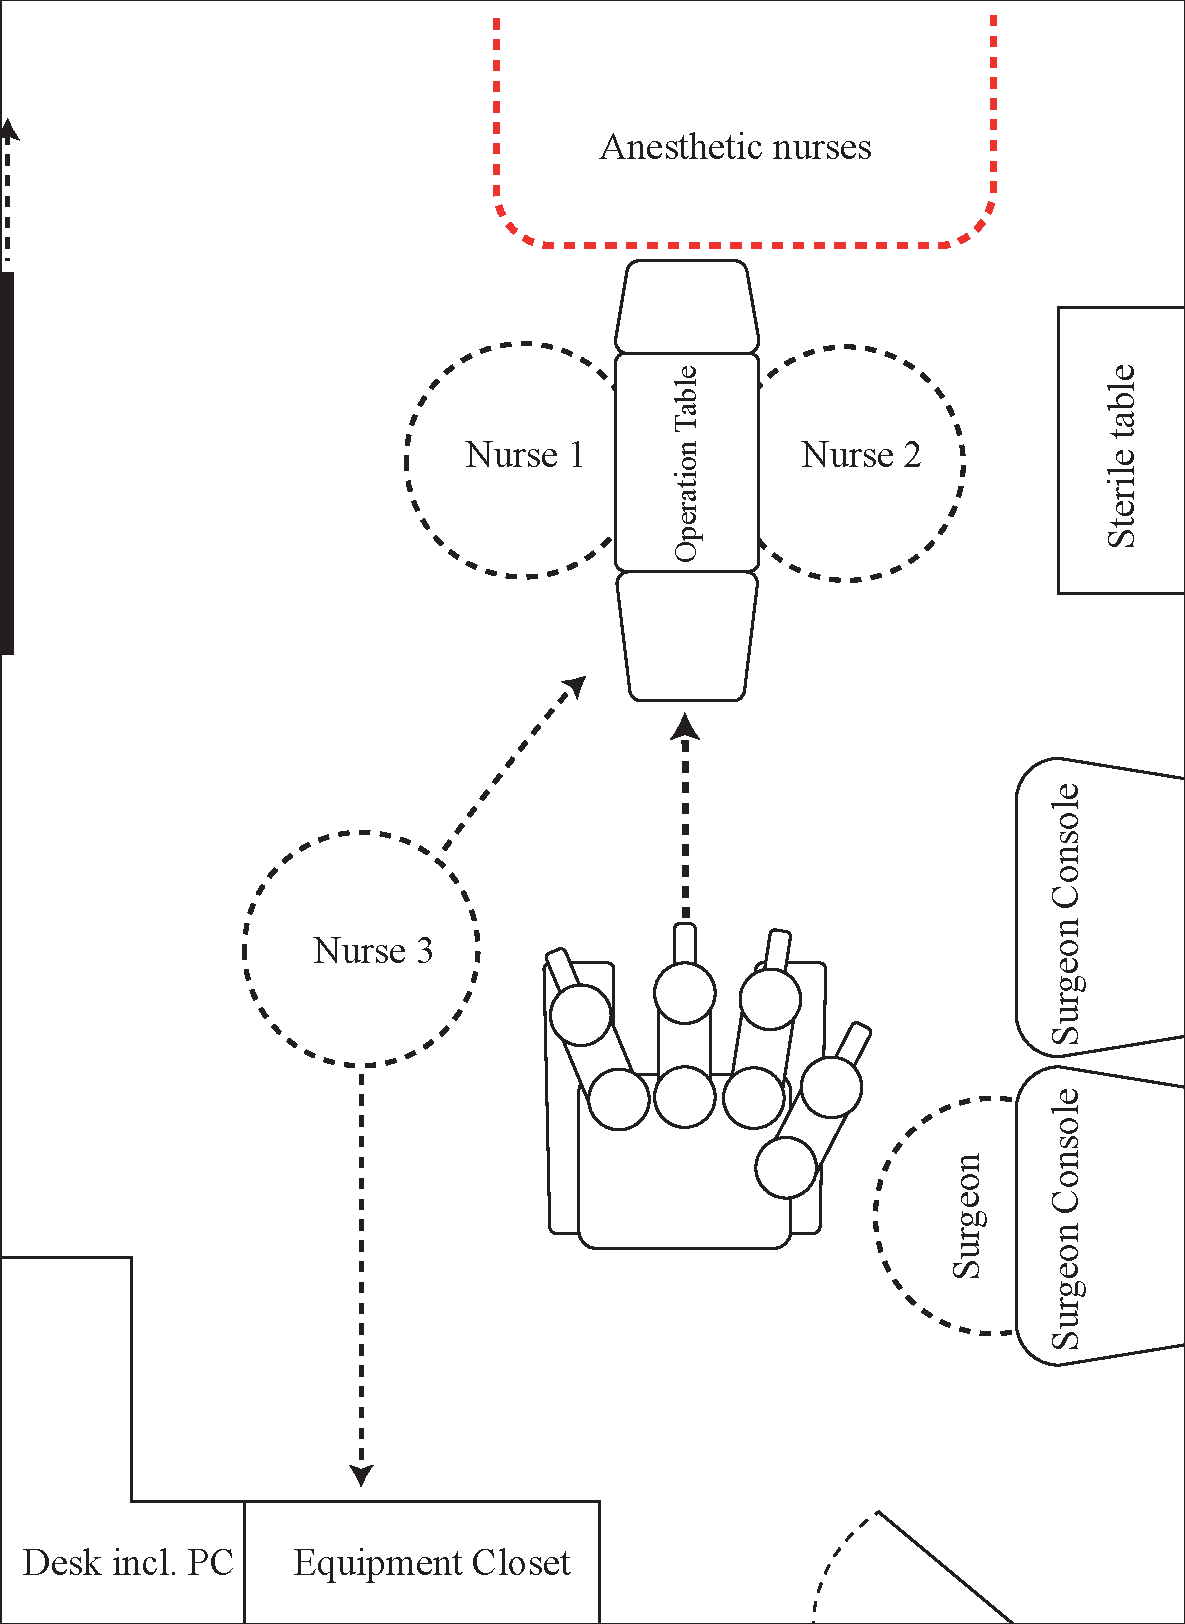
\includegraphics[width=\textwidth]{physical}
	\caption{The phyiscal model showing the layout of the operation room.}
	\label{fig:layout}
\end{figure}

This enables the development and design of the room when creating the simulation.\\

The sequence model is made from the the handed out paper "Teoretisk og praktisk undervisning ved robotten som følgende". The sequence model is shown in \autoref{fig:sequence}.

\begin{figure}[hbpt]
	\centering
	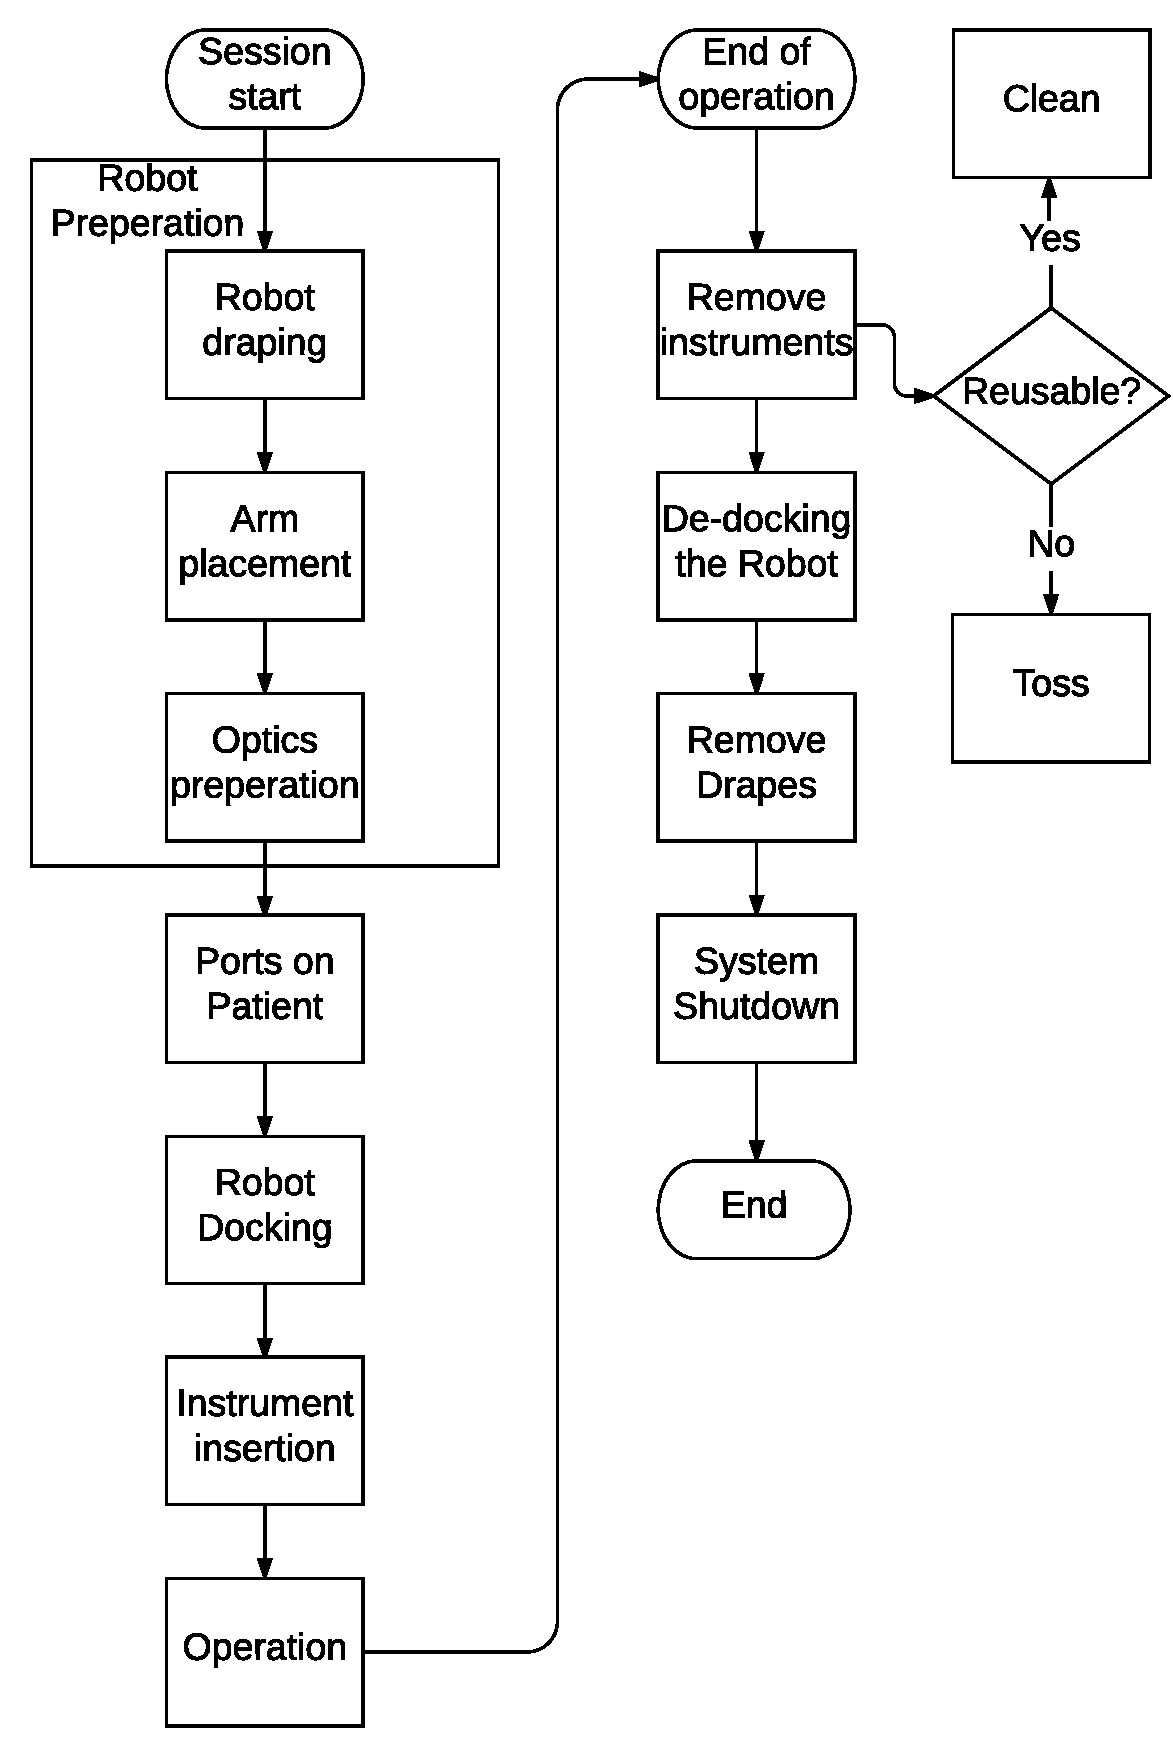
\includegraphics[width=0.6\textwidth]{sequencemodel}
	\caption{Flowchart of the sequence model showing how the operation preparation and debrief is carried out.}
	\label{fig:sequence}
\end{figure}

The sequence model describes the actions necessary to both start the operation and to end it. This enables the design of the tasks which should be included in the simulation and their order of appearance to the user.
The model shown is for an operation without any complications which could lead to de-docking of the robot in an emergency.\\


The Artefact models are shown in \autoref{fig:artefacts}. These are created from pictures taken at the observation of the operation. \autoref{fig:drapes} shows the drapes used to cover the arms of the robot sterilising the robot. \autoref{fig:camera} shows the camera also known as the endoscope and calibration equipment.

\begin{figure}[hbpt]
	\centering
	\begin{subfigure}[b]{0.4\textwidth}
		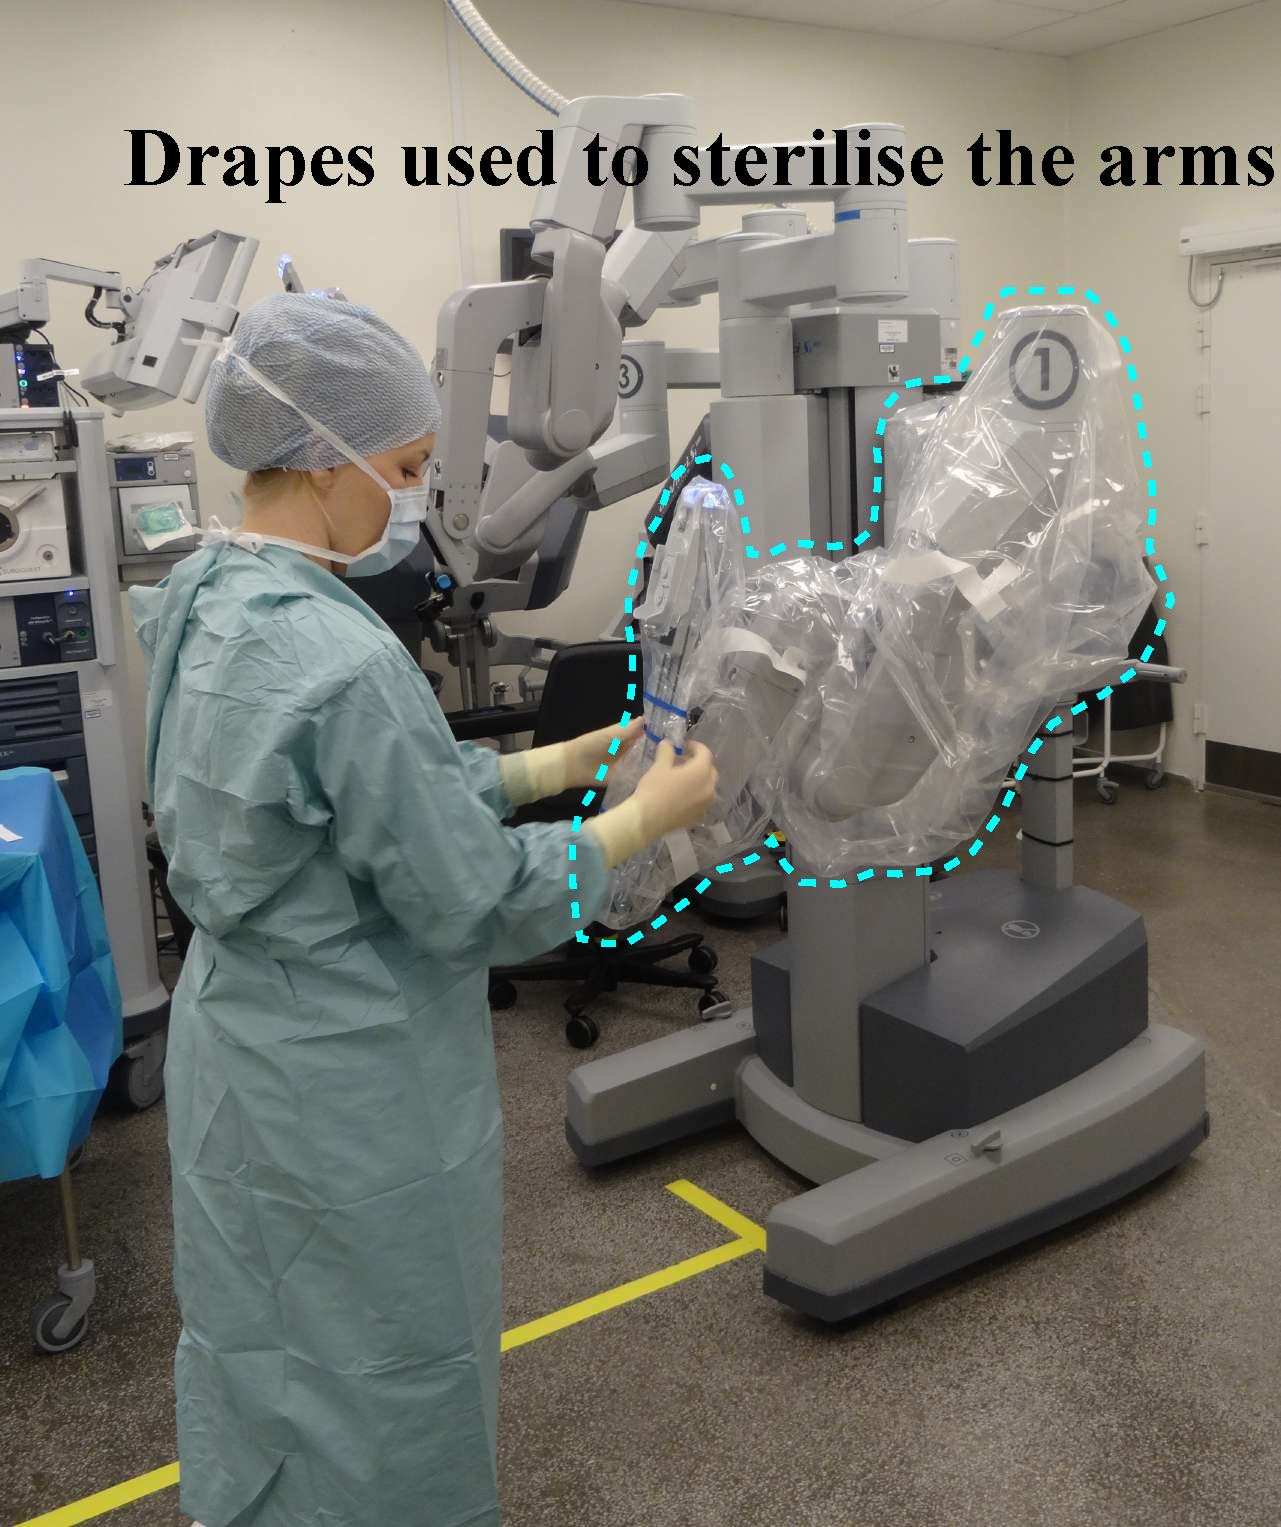
\includegraphics[width=\textwidth]{drapes}
		\caption{Figure showing the drapes used to cover the arms of the robot, sterilising them.}
		\label{fig:drapes}
	\end{subfigure}
	\begin{subfigure}[b]{0.4\textwidth}
		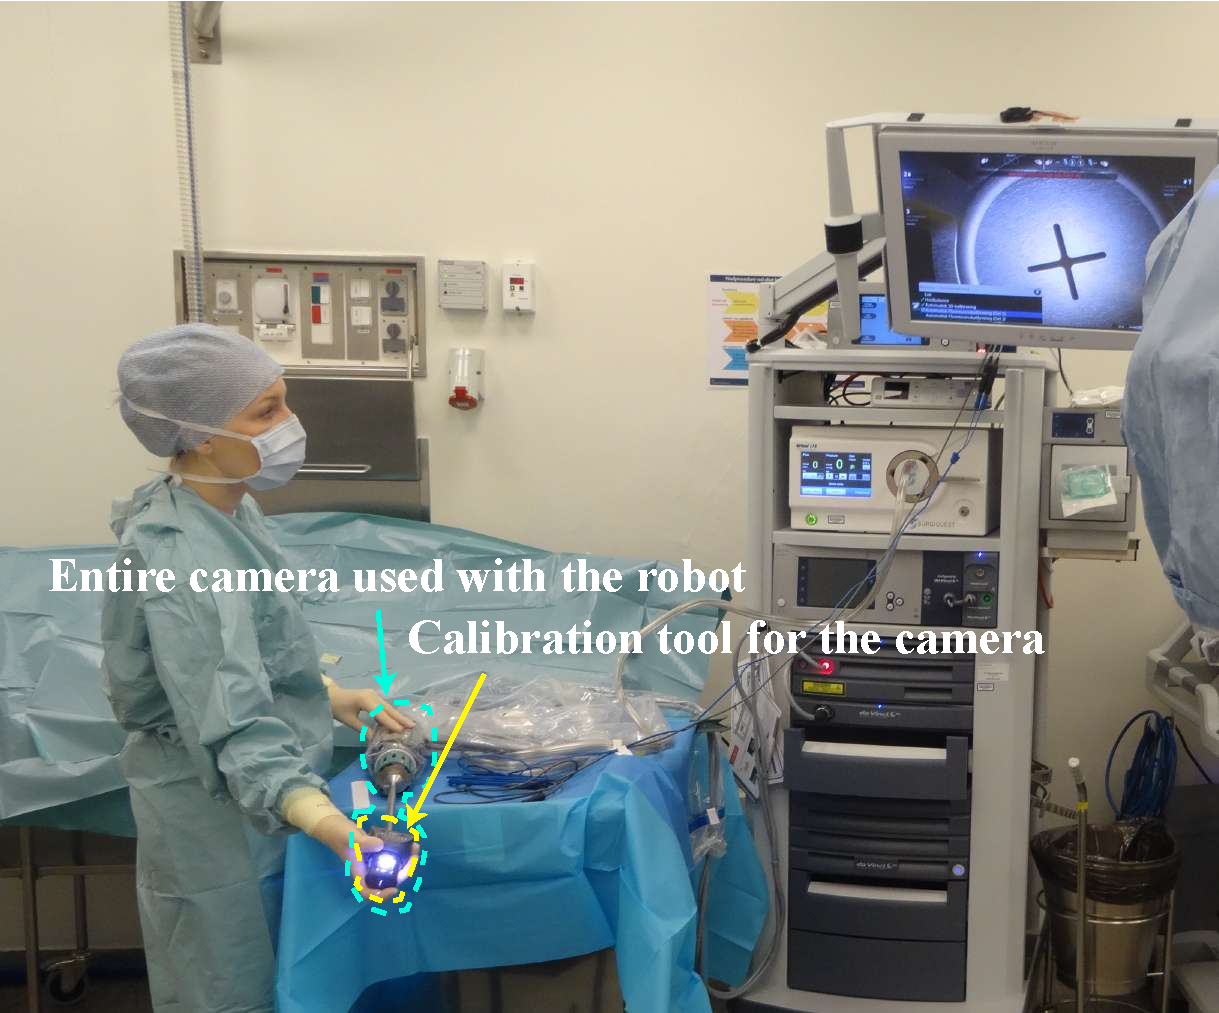
\includegraphics[width=\textwidth]{camera}
		\caption{Figure showing the camera used with the robot and a calibration tool.}
		\label{fig:camera}
	\end{subfigure}
	\caption{The figures show the artefacts used with the robot.}
	\label{fig:artefacts}
\end{figure}

\section{Conclusion}
The physical model yields both information regarding the physical layout of the simulation which must be develop as well as limiting of the scenarios which can be implemented. 

The sequence model outlines the entire scenario in which the tasks must be implemented as well as yielding an overview of what is crucial to include in the simulation.

The artefact model also shows which tools are important for the simulation to work as intended.

\newpage

\appendix % Start of appendix
\section{Notes Taken During the Observation}
\begin{itemize}
	\item If you are not sterile, you have to satnad at least one meter from sterile objects.
	\item The tables covered in green paper blankets are sterile.
	\item When preparing tools and unpacking, two nurses works together. One non-sterile nurse unpacks while the other, sterile, nurse grabs and places the tools on the sterile table.
	\item The sterile nurse sterilises the robot.
	\item When the patient enters the room he is firstly laid down on the operating table and then prepared for surgery.
	\item The stereoscopic camera is wrapped separately from the robot and other tools.
	\item When all sterile tools are placed, the sterile table is covered.
	\item The camera is calibrated by the sterile nurse. This is done using different kinds of end pieces and rotating them around scopes.
	\item The arms of the robot must be placed in a specific order. This is to avoid any kind of collision of the arms. Furthermore, the placement of the arms is as important as the order. This is done before the robot is docked.
	\item  Before the robot is docked, the nurses taking part in the operation are sterilising.
	\item When the robot is docked the arms are once again placed, this time around the ports inserted on the patient.
	\item A time out is taken before any cutting securing everyone and everything is ready and in place.
	\item The first cut done on the patient is to expand his stomach using air, easing the operation as this will yield more space.
	\item Before docking the camera on the robot it is used hand held to insert the other instruments and afterwards docked on the dedicated robot arm.
	\item When the camera is docked the robot arms are placed as far apart as possible. This is done to avoid collision.
	\item Each arm has three buttons enabling arm movement in two different ways.
	\item Cleaning of the optics is done several times during the operation. it may even be changed for another if it is too dirty.
	\item Communication during operation is somewhat an issue as the original speaker system made for this kind of surgery is broken. Instead, a small speaker and bad microphone is used.
\end{itemize}


\end{document}